\subsection{Model Performance Overview}
\label{subsec:pmc-results-model-performance-overview}

This section evaluates the ability of regression models to estimate peak memory usage from shape parameters.
Given the earlier evidence of near-linear scaling with volume, the primary focus is whether different algorithms can reliably reproduce this relationship.

Nine regression models were tested on Envelope, \ac{GST3D}, and Gaussian Filter.
Performance was measured using \ac{RMSE}, \ac{MAE}, $R^2$, and a combined ranking \textit{score}, as defined in Section~\ref{sec:pmc-materials-and-methods}.

\begin{figure*}[htbp]
    \centering
    \begin{subfigure}[t]{0.49\textwidth}
        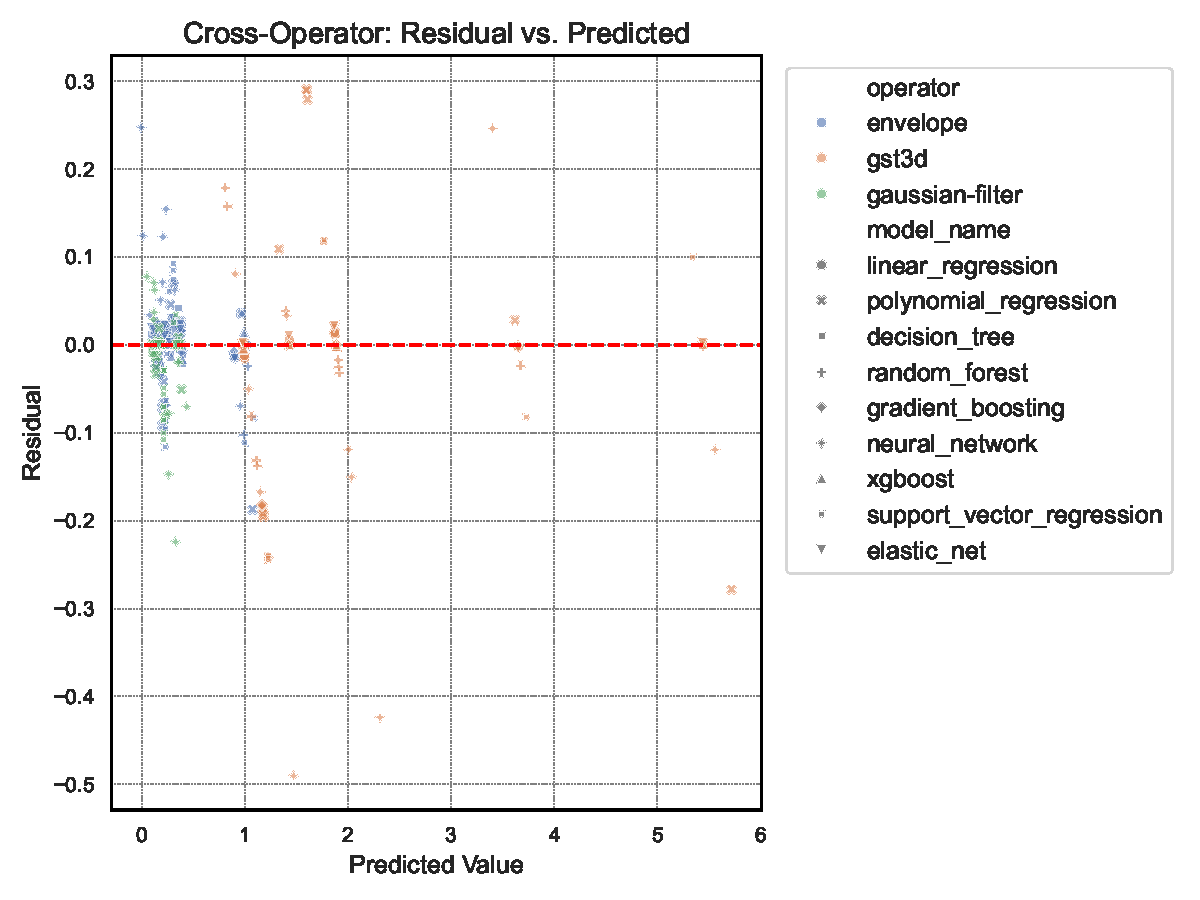
\includegraphics[width=\textwidth]{assets/images/05/residual_vs_predicted}
        \caption{Residual vs. predicted values (GB)}
    \end{subfigure}
    \hfill
    \begin{subfigure}[t]{0.49\textwidth}
        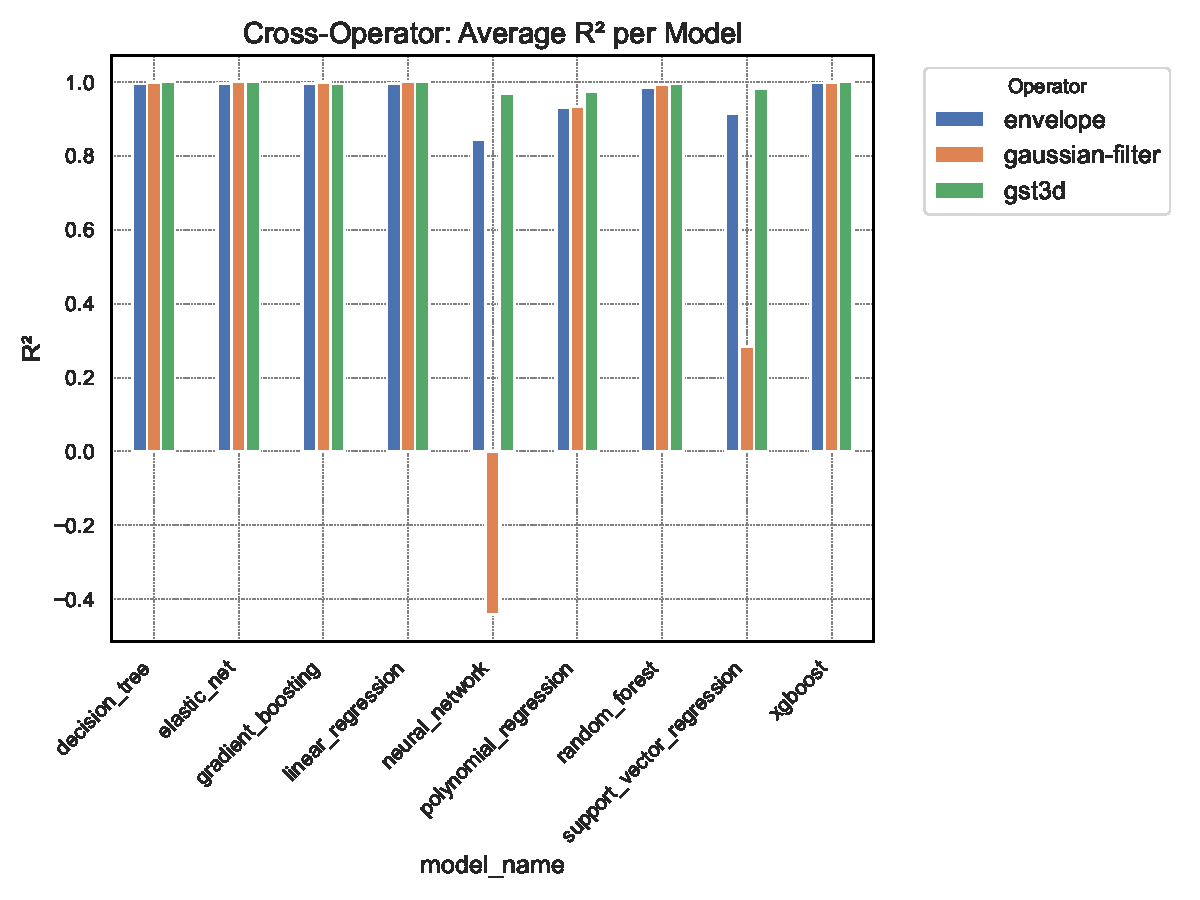
\includegraphics[width=\textwidth]{assets/images/05/cross_model_r2_bar}
        \caption{$R^2$ scores}
    \end{subfigure}
    \caption{Residual errors and $R^2$ for all models and operators. Simpler models (Linear Regression, Elastic Net) consistently yield high $R^2$.}
    \label{fig:residual_vs_predicted_and_r2_bar}
\end{figure*}

Table~\ref{tab:performance_summary} highlights the best-performing model per operator.

\begin{table}[htbp]
    \centering
    \begin{tabular}{lccc}
        \hline
        \textbf{Operator} & \textbf{Best Model} & \textbf{Score} & \textbf{Note}                \\
        \hline
        Envelope          & Gradient Boosting   & 2.579          & Low RMSE, stable predictions \\
        \ac{GST3D}        & Decision Tree       & 2.970          & Top $R^2$, low residuals     \\
        Gaussian Filter   & Linear Regression   & 2.904          & Similar to Elastic Net       \\
        \hline
    \end{tabular}
    \caption{Top models by score for each operator.}
    \label{tab:performance_summary}
\end{table}

Figure~\ref{fig:actual_vs_predicted} confirms that these models closely align with actual memory values.

\begin{figure*}[htbp]
    \centering
    \begin{subfigure}[t]{0.32\textwidth}
        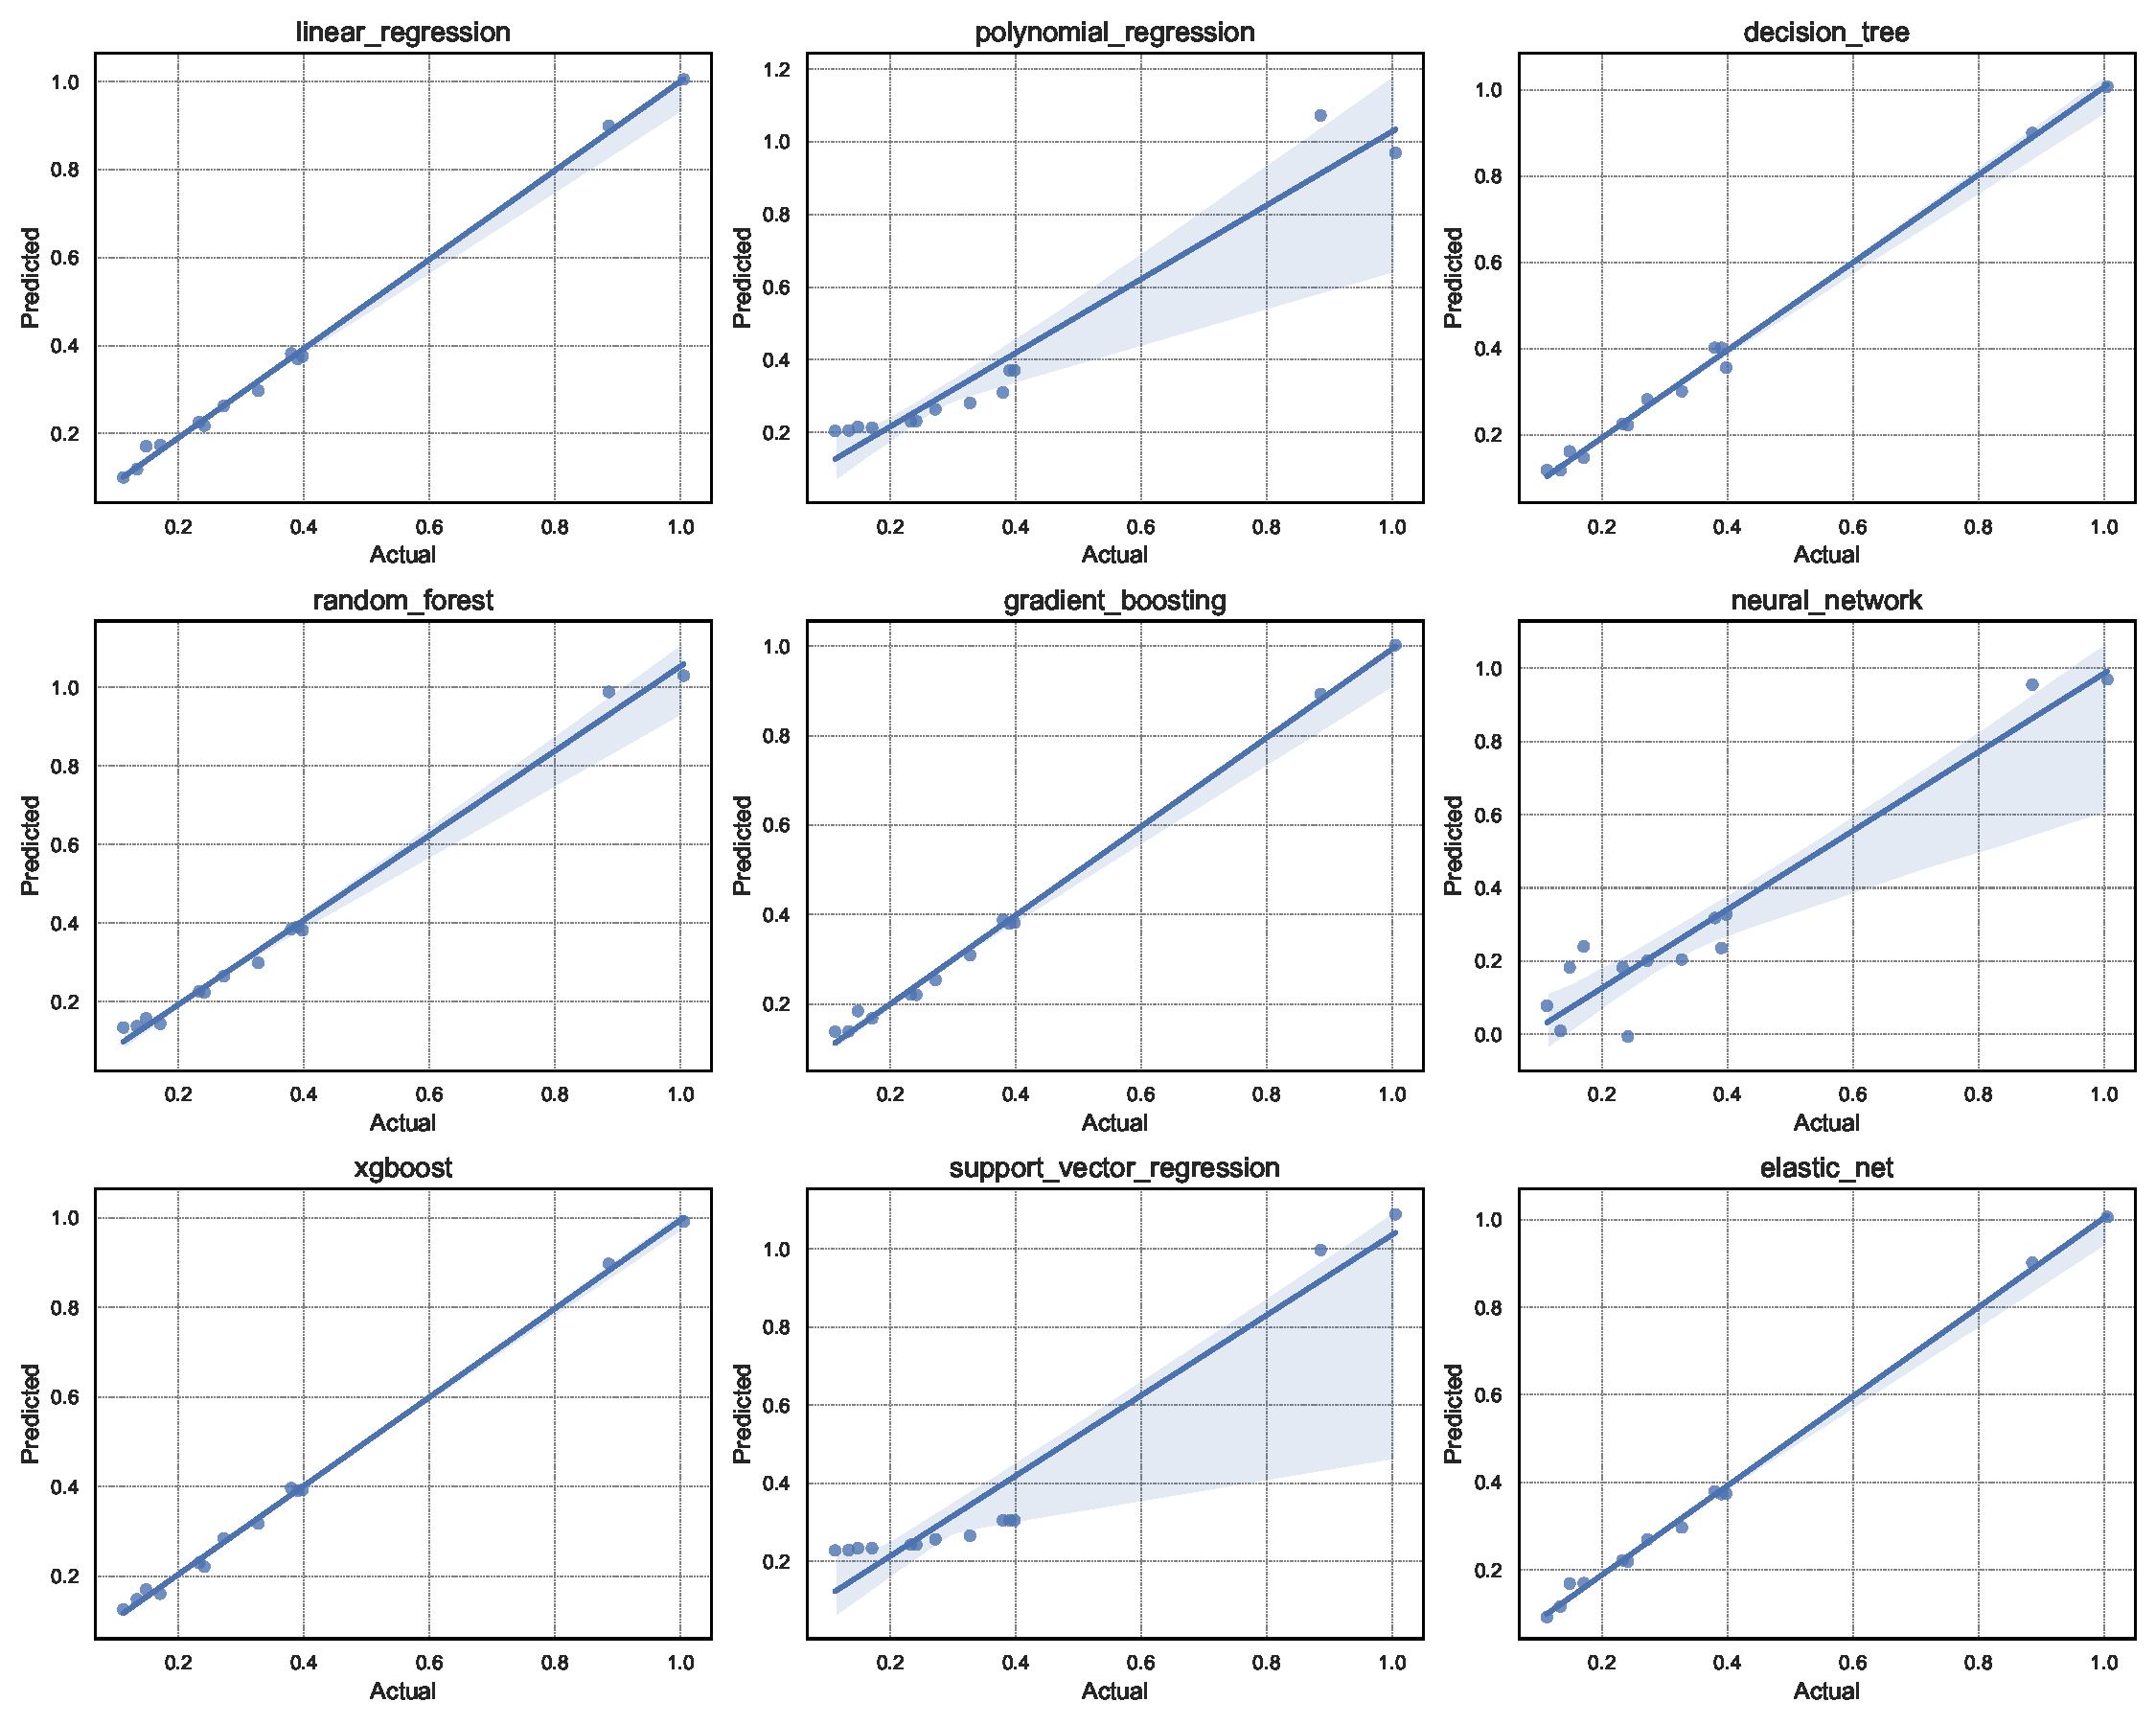
\includegraphics[width=\textwidth]{assets/images/05/actual_vs_predicted_by_model_envelope}
        \caption{Envelope}
    \end{subfigure}
    \hfill
    \begin{subfigure}[t]{0.32\textwidth}
        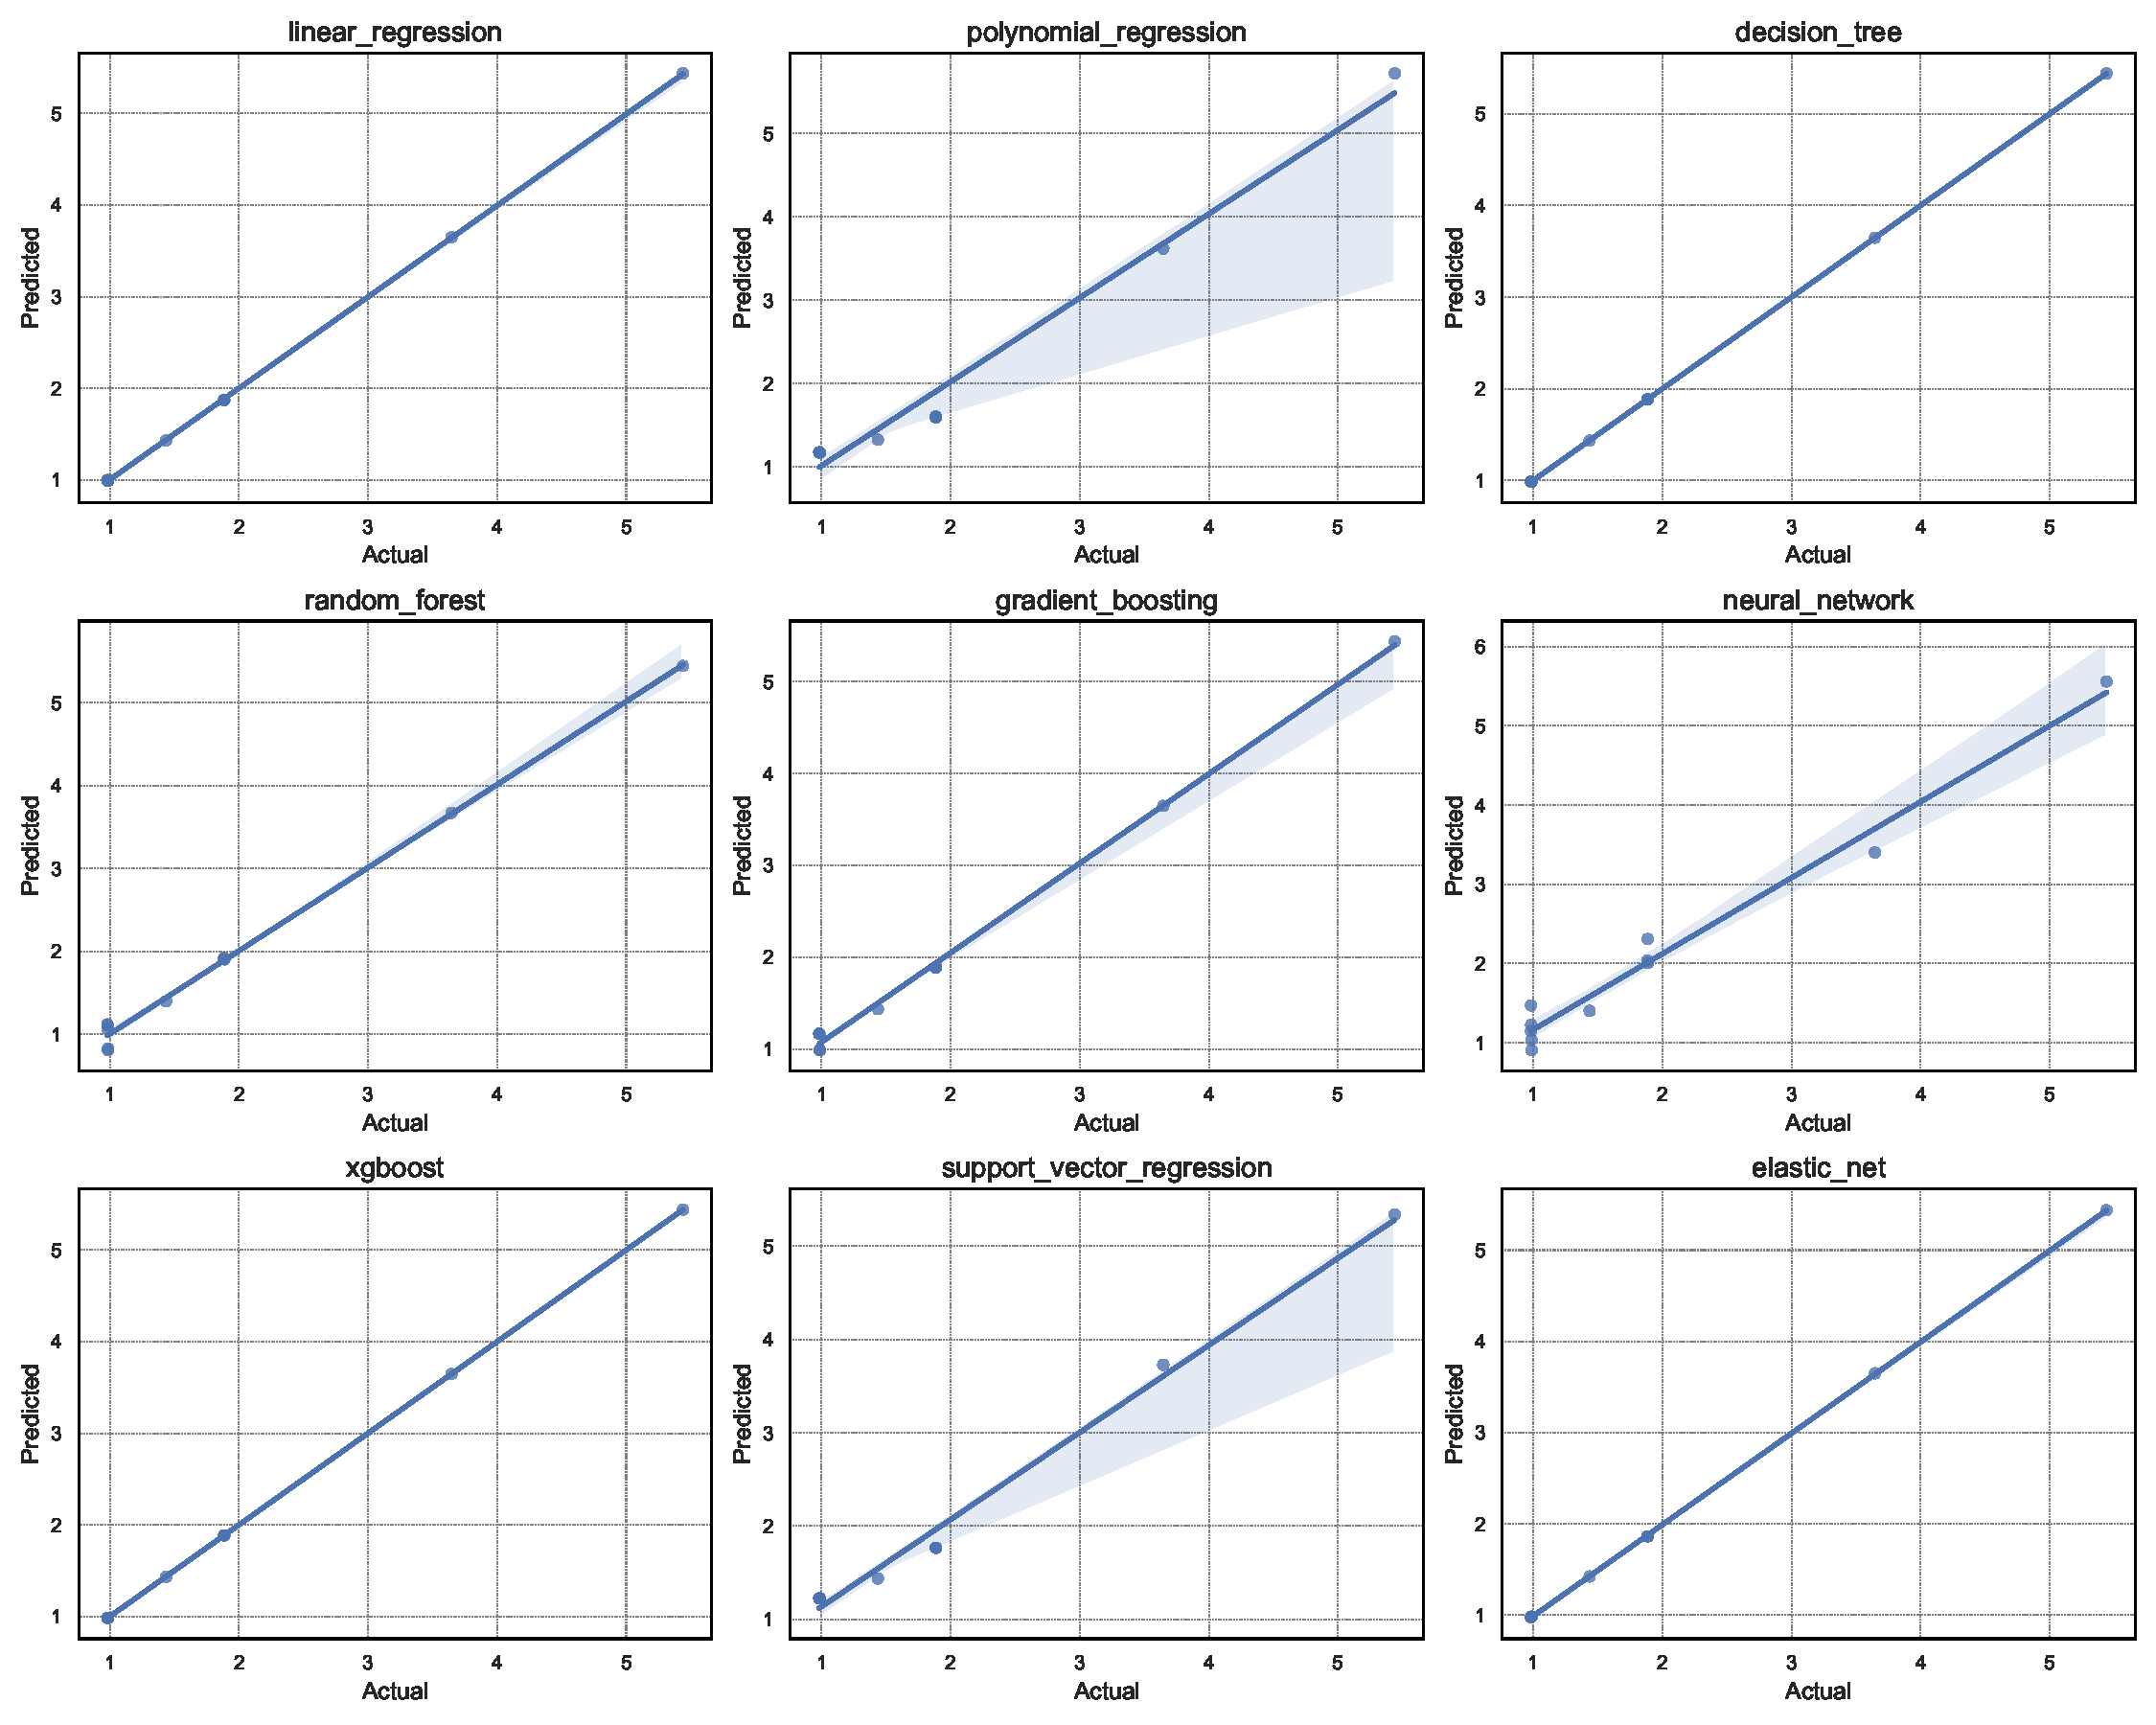
\includegraphics[width=\textwidth]{assets/images/05/actual_vs_predicted_by_model_gst3d}
        \caption{\ac{GST3D}}
    \end{subfigure}
    \hfill
    \begin{subfigure}[t]{0.32\textwidth}
        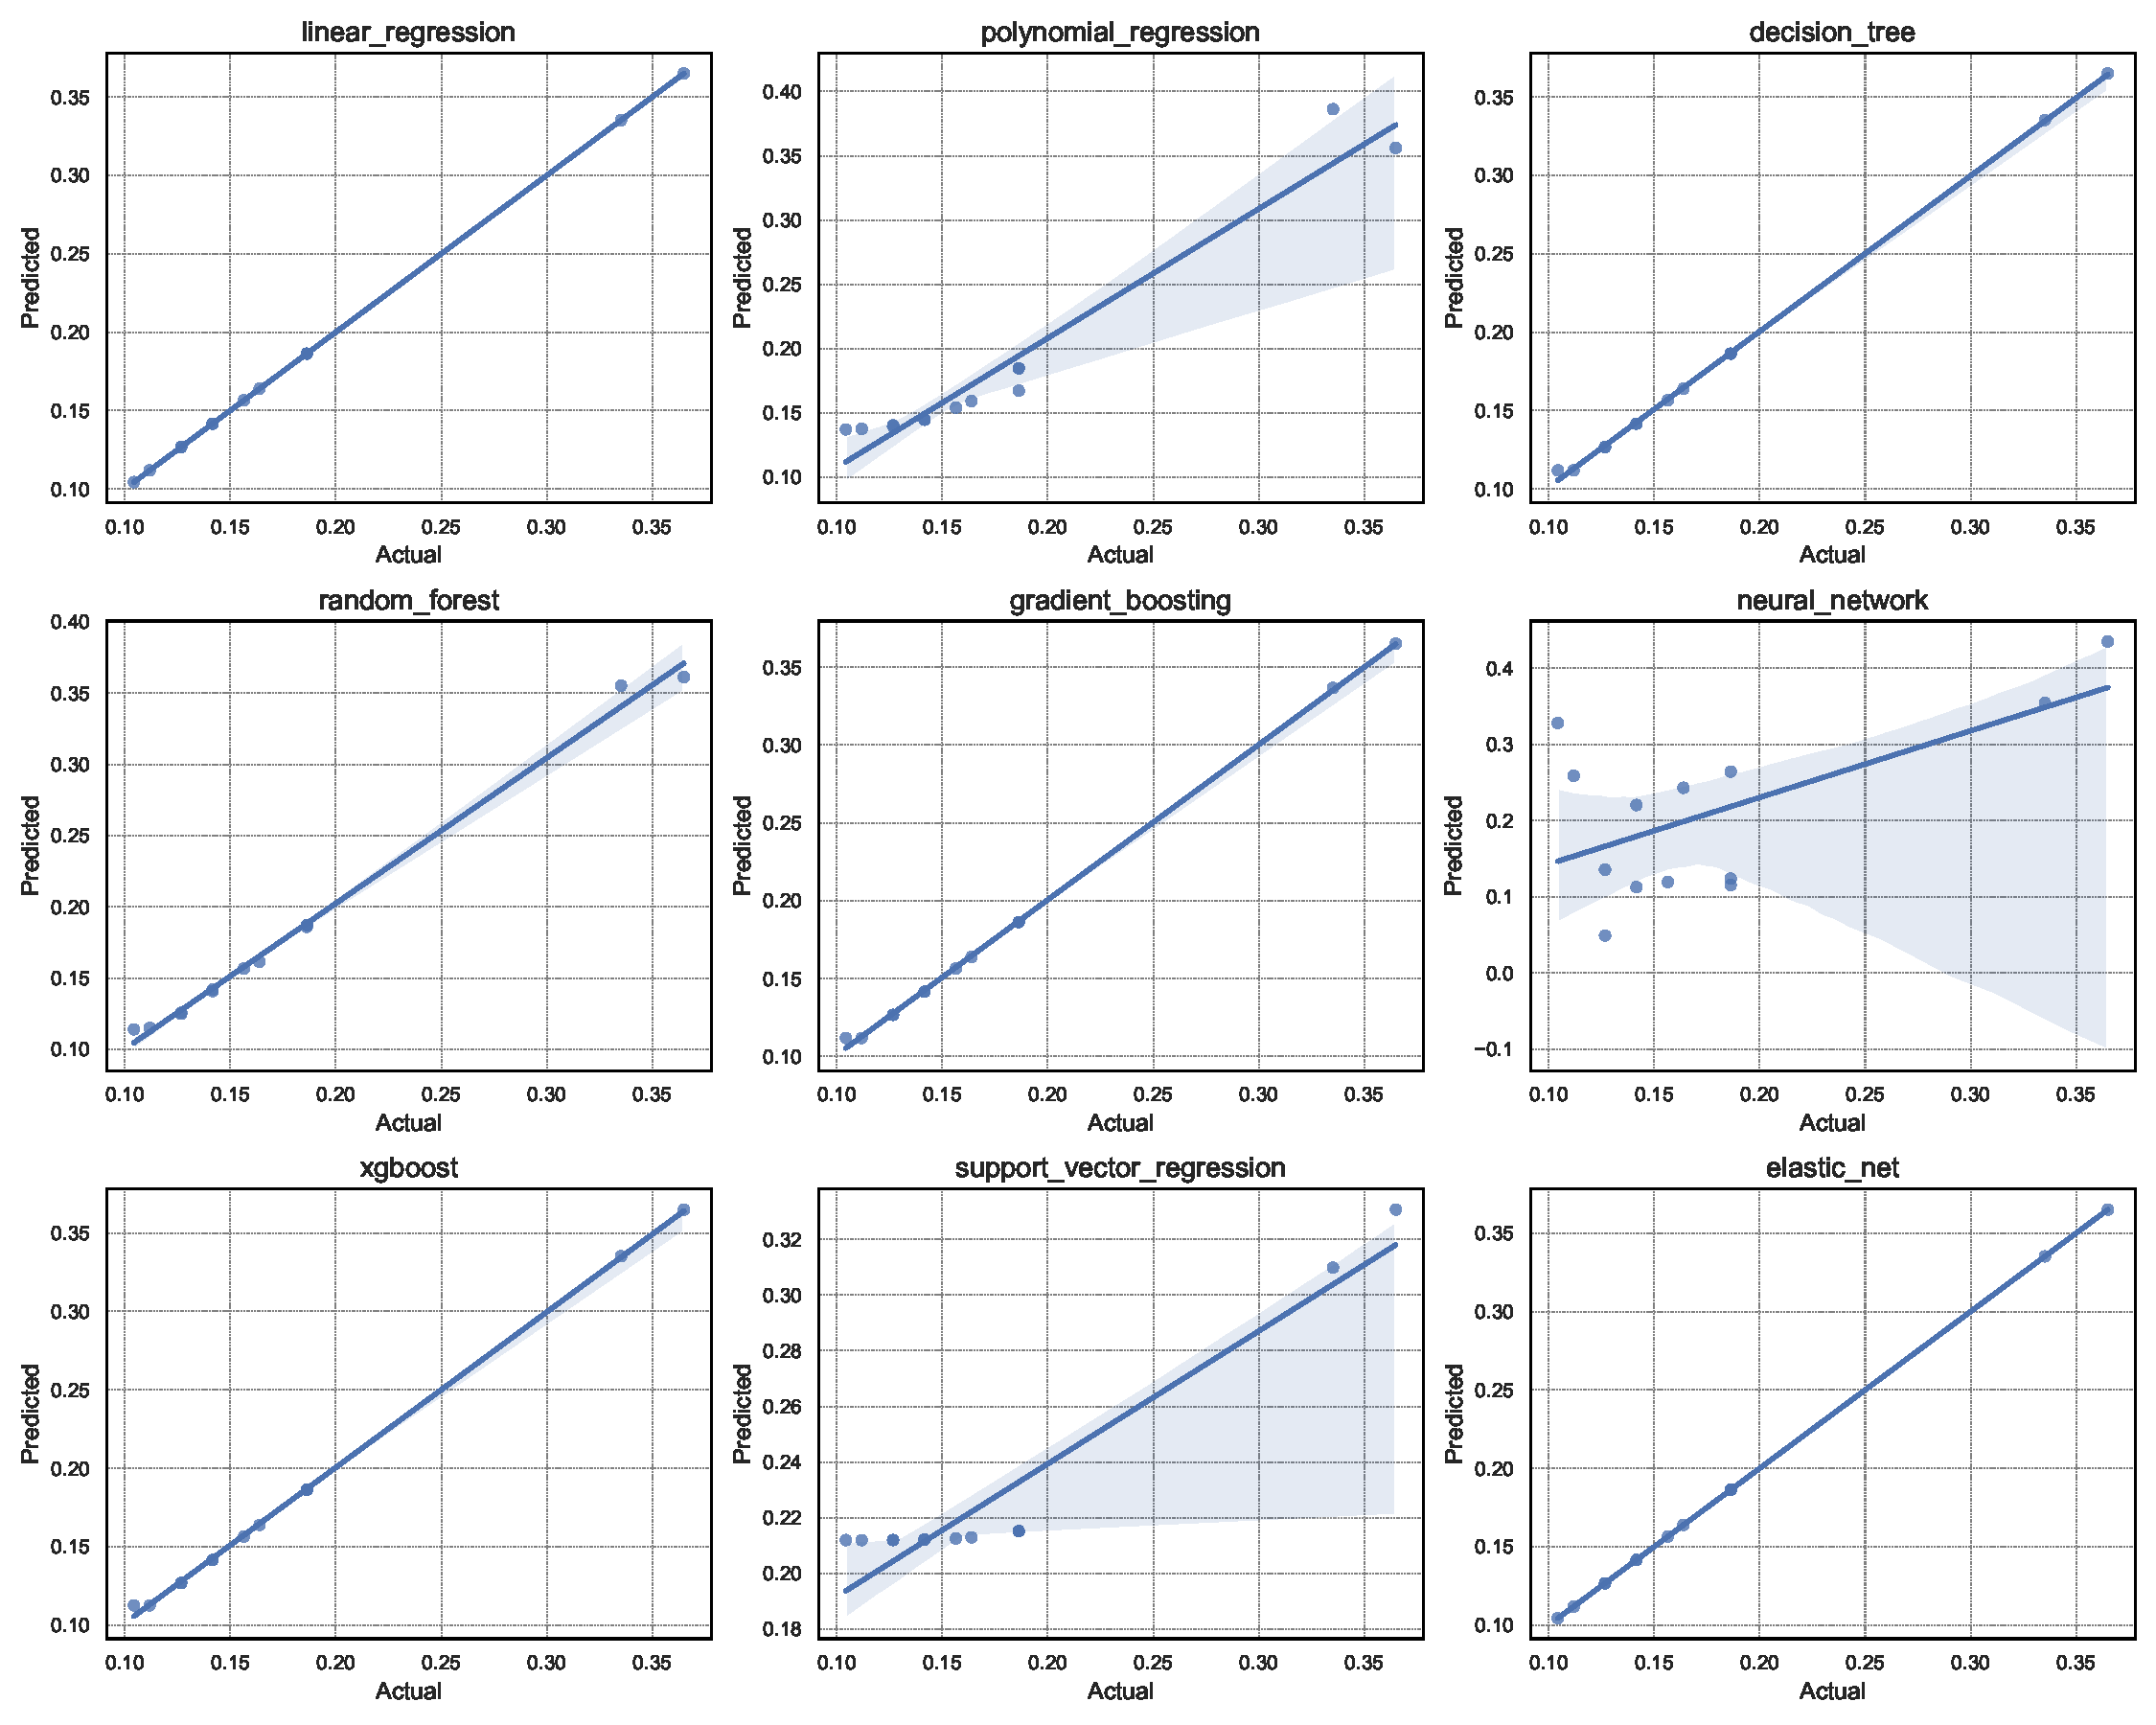
\includegraphics[width=\textwidth]{assets/images/05/actual_vs_predicted_by_model_gaussian-filter}
        \caption{Gaussian Filter}
    \end{subfigure}
    \caption{Actual vs. predicted memory usage. Strong alignment across most models, especially for Envelope and Gaussian Filter.}
    \label{fig:actual_vs_predicted}
\end{figure*}
